\section{Theorie}
\label{sec:Theorie}
Brückenschaltungen werden genutzt um größen zu vermessen, die sich als elektrische Wiederstände darstellen lassen. Dazu zählen auch
komplexe Widerstände, wie die von Spulen und Kondensatoren.
Grundsätzlich bestehen Brückenschaltungen aus vier Widerständen, wie in Abbildung \ref{fig:einfachbruecke}.
Es kann die Brückenspannung an den Punkten $A$ und $B$ abgegriffen werden.
\begin{figure}
 \centering
 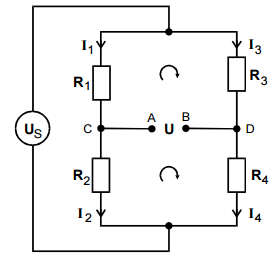
\includegraphics[width=0.4\textwidth]{bruecke.PNG}
 \caption{Aufbau einer einfachen Brückenschaltung.\cite{sample}}
 \label{fig:einfachbruecke}
 \end{figure}\\
Mit den Kirchhoffschen Regeln:
 \begin{align}
  \intertext{1. Die Summe aller eingehenden und abgehenden Ströme an einem Knoten ist gleich Null:}
  \sum_k I_\mathrm{k}&=0
  \intertext{2. Die Summe der Spannungen in einer Masche ist, unter Beachtung des Vorzeichens, gleich Null:}
  \sum_k U_\mathrm{k}&=0
  \intertext{und dem Ohmschen-Gesetzt:}
  U&=R\cdot I
 \end{align}
 ergibt sich für die Brückenspannung:
 \begin{align}
   U_\mathrm{Br}=\frac{R_\mathrm{2} R_\mathrm{3}- R_\mathrm{1} R_\mathrm{4}}{(R_\mathrm{3}+R_\mathrm{4})+(R_\mathrm{1}+R_\mathrm{2})}\cdot U_\mathrm{S}\label{eqn:verhältnis}.
 \end{align}
Dieser Ausdruck ist lediglich von den Schaltungsparametern abhängig und
verschwindet unabhängig von der Speisespannung $U_\mathrm{S}$, wenn gilt:
\begin{align}
  R_\mathrm{1}R_\mathrm{4}=R_\mathrm{2}R_\mathrm{3}.
\end{align}
Dieser Zusammenhang bezeichnet die abgeglichene Brücke, damit ist eine
Widerstandsmessung möglich. Ist Einer der Widerstände unbekannt, kann
mindestens ein Anderer so variiert werden bis die Brückenspannung verschwindet,
aus dem Verhältnis kann der unbekannte Widerstand bestimmt werden.
\subsection{Wheatstonesche Brücke}
\begin{figure}
 \centering
 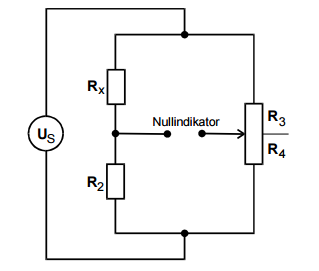
\includegraphics[width=0.4\textwidth]{wheat.PNG}
 \caption{Aufbau Wheatstonesche Brücke.\cite{sample}}
 \label{fig:wheat}
 \end{figure}
In der Abbildung \ref{fig:wheat} findet sich der Aufbau einer Wheatstoneschen Brücke, diese besteht nur aus ohmschen Widerständen.
Anstelle von $R_\mathrm{1}$ wird hier ein unbekannter Widerstand $R_\mathrm{X}$ verwendet.
Nach Formel \eqref{eqn:verhältnis} gilt für $R_\mathrm{X}$:
\begin{align}
  R_\mathrm{X}=R_\mathrm{2}\frac{R_\mathrm{3}}{R_\mathrm{4}}.\label{eqn:Wheat}
\end{align}
$R_\mathrm{X}$ hängt nur vom Verhältnis $R_\mathrm{3}$ zu $R_\mathrm{4}$ ab, diese werden in diesem Versuch als Potentiometer realisiert.\\
\subsection{Kapazitätsmessbrücke}
Bei realen Kondensatoren treten Verluste in Form von Wärme auf, um dies bei Berechnungen zu berücksichtigen, wird zu seiner Kapazität ein fiktiver Ohmscher Widerstand in Reihe geschaltet.
\begin{figure}
 \centering
 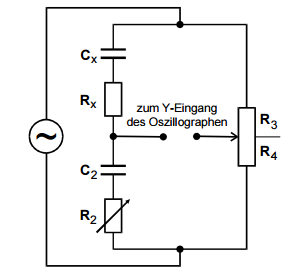
\includegraphics[width=0.4\textwidth]{kapazitaet.PNG}
 \caption{Aufbau einer Kapazitätsmessbrücke.}
 \label{fig:kapazitaet}
 \end{figure}
In Abbildung \ref{fig:kapazitaet} ist eine Kapazitätsmessbrücke dargestellt. Diese besteht aus einer unbekannten Kapazität $C_\mathrm{X}$,
einem unbekannten Widerstand $R_\mathrm{X}$, einer bekannten Kapazität $C_\mathrm{2}$ und zum Ausgleich, von der von $R_\mathrm{X}$ verursachten Phasenverschiebung,
ein variabler Widerstand $R_\mathrm{2}$.
Es gilt:
\begin{align}
  R_\mathrm{X}&=R_\mathrm{2}\frac{R_\mathrm{3}}{R_\mathrm{4}}\label{eqn:CR}\\
  C_\mathrm{X}&=C_\mathrm{2}\frac{R_\mathrm{4}}{R_\mathrm{3}}\label{eqn:CC}.
\end{align}\\
\subsection{Induktivitätsmessbrücke}
\begin{figure}
 \centering
 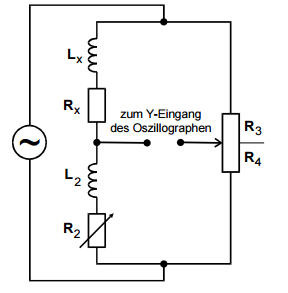
\includegraphics[width=0.4\textwidth]{induktivitaet.PNG}
 \caption{Aufbau einer Induktivitätsmessbrücke.}
 \label{fig:induktivitaet}
 \end{figure}
 In Abbildung \ref{fig:induktivitaet} ist eine Induktivitätsmessbrücke zu sehen, die ist ähnlich aufgebaut wie die Kapazitätsmessbrücke,
 nur werden die Kapazitäten durch Induktivitäten ausgetauscht.
 Weil die komplexen Widerstände von Induktivitäten anders definiert sind als die der Kapazitäten, ergeben sich andere Formeln für $R_\mathrm{X}$ und $L_\mathrm{X}$:
 \begin{align}
   R_\mathrm{X}=R_\mathrm{2}\frac{R_\mathrm{3}}{R_\mathrm{4}}\label{eqn:LR}\\
   L_\mathrm{X}=L_\mathrm{2}\frac{R_\mathrm{3}}{R_\mathrm{4}} \label{eqn:LL}
 \end{align}
\subsection{Maxwell-Brücke}
\label{sec:Max}
Die Maxwell-Brücke wird ebenfalls zur Induktivitätsmessung genutzt.
Hierbei wird auf die bekannte Induktivität $L_\mathrm{2}$ verzichtet, stattdessen wird ein Kapazität $C_\mathrm{4}$ verwendet, diese ist verlustärmer als eine Spule.
\begin{figure}
 \centering
 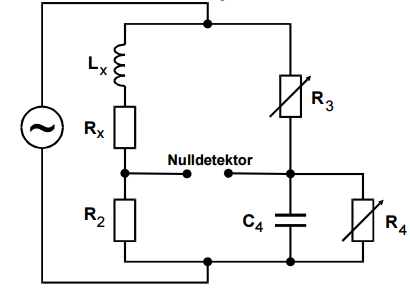
\includegraphics[width=0.4\textwidth]{maxwell.PNG}
 \caption{Aufbau einer Maxwell-Brücke.\cite{sample}}
 \label{fig:maxwell}
 \end{figure}
Für $L_\mathrm{X}$ und $R_\mathrm{X}$ gilt:
\begin{align}
  R_\mathrm{X}&=\frac{R_\mathrm{2}R_\mathrm{3}}{R_\mathrm{4}}\label{eqn:RM}\\
  L_\mathrm{X}&=R_\mathrm{2}R_\mathrm{3}C_\mathrm{4}\label{eqn:LM}
\end{align}
\subsection{TT-Brücke}
Die TT-Brücke, zu sehen in Abbildung \ref{fig:tt}, wird als elektronischer Filter genutzt.
In diesem Versuch dient die Brücke zum filtern von Schwingungen mit der Frequenz $\omega_0$, ebenfalls schwächt sie Schwingungen die in der Nähe liegen stark ab.
In dem Aufbau gibt es keine Abgleichelemente, alle Eigenschaften der Bauteile sind festgelegt.
\begin{figure}
 \centering
 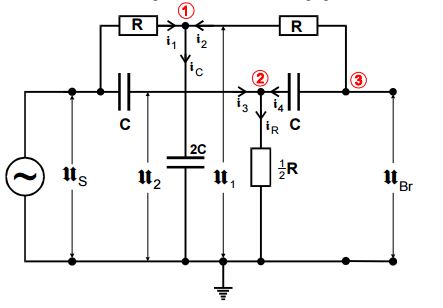
\includegraphics[width=0.5\textwidth]{tt.PNG}
 \caption{Aufbau einer TT-Brücke.\cite{sample}}
 \label{fig:tt}
 \end{figure}
Für die Brückenspannung gilt:
\begin{align}
  U_\mathrm{Br}=U_\mathrm{S}\frac{1-\omega^2 R^2 C^2}{1-\omega^2 R^2 C^2 + 4j \omega R C}\label{eqn:ubr}.
\end{align}
Für die Frequenz $\omega_0=\frac{1}{RC}$ verschwindet die Brückenspannung.
Mit der normierten Frequenz $\Omega:=\frac{\omega}{\omega_0}$ und weiteren Umformungen gilt:
\begin{align}
  \left|\frac{U_\mathrm{Br}}{U_\mathrm{S}}\right|=\sqrt{\frac{\left(\Omega^2-1\right)^2}{\left(1-\Omega^2\right)^2+16\Omega^2}}\label{eqn:TT}.
\end{align}
\subsection{Klirrfaktor}
Als Klirrfaktor wird der Anteil von Oberwellen im Verhältnis zur Grundwelle bezeichnet. Oberwellen werden ungewollt generiert, wenn Sinusschwingungen synthetisiert werden.
Für das Verhältnis gilt:
\begin{align}
  k=\frac{sqrt{U_2^2+U_3^2+...}}{U_1}\label{eqn:klirr}.
\end{align}
